% !TEX root=/home/tavant/these/manuscript/src/manuscript.tex

\section{Validation of the sheath model }
  \label{sec-sheath_validation}
  
  The \ac{PIC} simulations used here do not need any sheath theory in order to model the plasma-wall interaction.
  Conversely, they rely on first principle models.
  Hence, they can be used in order to validate the sheath modeled introduced in \cref{sec-sheath} coming from the fluid theory.
  
  This sheath model links with \cref{eq-sheathhobbs} the plasma potential drop $\dphi$ with the electron temperature $\Te$ and the electron emission rate $\rate$.
  \inlinenote{Anne: pourquoi tu parles de 1.50 la ? Parler de 2.11 suffit non?}
  \Cref{eq-seemaxw} can be used to estimate the electron emission rate given the mean electron temperature measured in the simulations, corresponding statistically to the plasma bulk temperature.   
  In the \ac{PIC} simulations, $\rate$ can be computed using \cref{eq-seeyield} by counting the number of electrons attaining the wall and emitted during a time-step.
  We note \ratepic this measurement.
  \vspace{1em}
   
  \begin{figure}[hbtp]
    \centering
    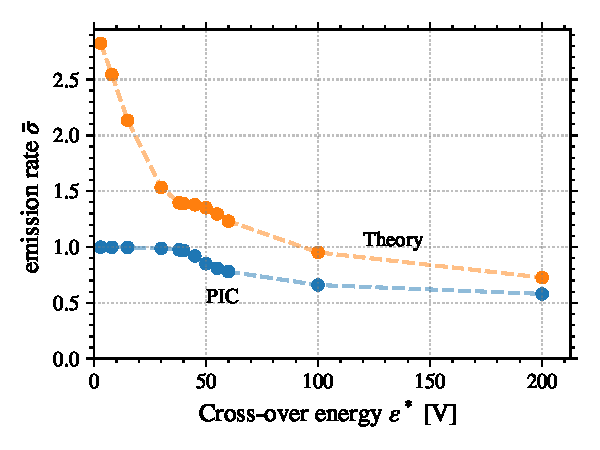
\includegraphics[width=\defaultwidth]{SEE_rates}
    \caption{Values of the electron emission rate $\ratepic$ (blue) measured in the \ac{PIC} simulations, and $ \ratemaxw$ obtained with \cref{eq-seemaxw} using the electron temperature shown in \cref{fig-Tevsproba}. }
    \label{fig-seeparamesMaxw}
  \end{figure}
  
  
  We can see in \Cref{fig-seeparamesMaxw} that the mean electron emission rate lies between 0.6 for large $\crover$ and 1 at low $\crover$.
  The saturation of \ratepic at 1 for high emissivity ( $\crover < 50 \volt$) was not expected from \ratemaxw.
  Indeed, \probamax is equal to 2.9, and the electron temperature in the bulk measured, when used in \cref{eq-seemaxw}, predicts a rate between 1.4 and 2.8.
  This discrepancy at low \crover is due to the \ac{SCL} regime.
  In \citet{hobbs1967}, the authors predict that in this regime, a potential well forms such that a fraction of the emitted electrons are returned to the wall, in order to maintain the effective emission rate to $\ratecr\sim1$.
  However, for $\crover > 50 \volt$, the sheath regime described in \cref{sec-sheath} should be valid.
   
  \begin{figure}[hbtp]
    \centering
    \begin{tabular}{cc}
      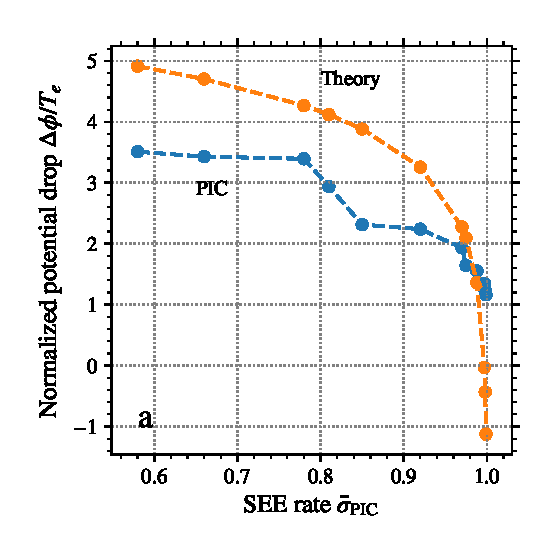
\includegraphics[width=3in]{phi_drop_6}
      &
      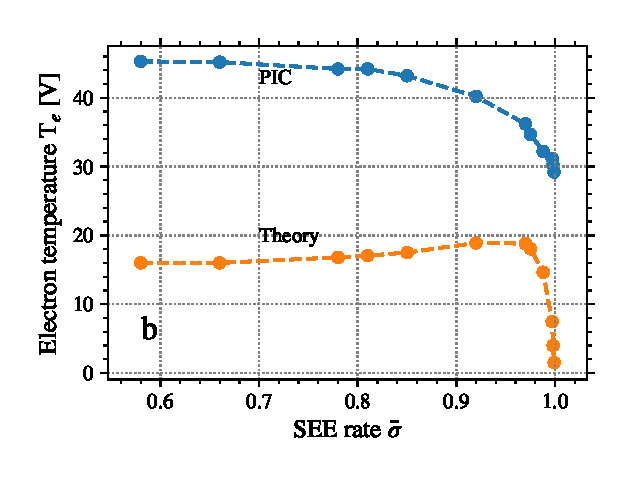
\includegraphics[width=3in]{Te_pic_2}
    \end{tabular}
    \caption{({\bf a}) Plasma potential drop to the wall normalized by the electron bulk as a function of the electron rate. {\bf $\Te$ is italic !}; ({\bf b}) Mean electron temperature measured in the \ac{PIC} simulations as a function of the electron emission rate \rate, measured as well in the simulations.  }
    \label{fig-Tevsproba}
  \end{figure}
  
  The electron temperature measured in the bulk of the simulation is presented in \cref{fig-Tevsproba}.{\bf b} for the same cases as in \cref{fig-seeparamesMaxw}.
  We can see that when \rate increases, $\Te$ monotonically decreases from 45V to around 30V.
  However, these values are not consistent with the measured emission rate \ratepic for $\crover > 50\volt$.

  \Cref{fig-Tevsproba}.{\bf a} shows the evolution of the potential drop to the wall measured in the \ac{PIC} simulation compared to the theory \vref{eq-total_drop} ({\bf OR is it \cref{eq-sheathhobbs} ...?}).
  As expected by \vref{eq-dphi_scl}, $\dphi$ measured in the simulation saturates to $\Te$ for high emission rate ($\ratepic \sim 1$).
  However, 
  We see that at low emission rate, the potential drop is significantly lower than expected.
  
  The sheath model of \cref{sec-sheath} used two hypotheses\string:
  \begin{itemize}
    \item Maxwellian electrons
    \item Isothermal evolution of the electrons
  \end{itemize}
  These two hypotheses will be confronted against the kinetic simulation in the next chapter.
  
  \inlinenote{Anne: bizarre dans la lecture: a la fin de la section 2.4, tu annonces 2 points importants et tu dis que tu vas en traiter 1 et on arrive a la fin de la section 2.5 avec 2 points d'hypotheses.....}
   